\chapter{Giới thiệu về Open World Assumption và Semantic Web}
\section{Open World Assumption}
Trước khi bắt đầu giới thiệu với sâu hơn về Ontology Web Language (OWL), chúng em xin được giới thiệu qua về giả định Thế Giới Mở (Open World Assumption - OWA)\cite{OWA_0} được Semantic Web chấp nhận và phân biệt giả định này với giả định Thế Giới Đóng (Closed World Assumption - CWA).
\begin{description}
\item[Closed World Assumption] 
Giả định Thế Giới Đóng (CWA) là giả định mà những điều không chắc hoặc không có cơ sở để chứng minh là \textbf{đúng} sẽ được chấp nhận là \textbf{sai}.
\item[Open World Assumption]
Giả định Thế Giới Mở (OWA) thì ngược lại, với những điều không chắc hoặc không có cơ sở để chứng minh là \textbf{đúng} sẽ được chấp nhận là \textbf{chưa biết}. 
\item[Ví dụ]
Xem xét một câu nói sau đây: "A là một công dân của nước Hoa Kỳ". Nếu có ai đó hỏi "A có phải là một công dân của Việt Nam hay không ?". Xét theo CWA, câu trả lời là \textit{không}, ngược lại với OWA thì câu trả lời là \textit{chưa biết}. 
\end{description}
\subsection{Vậy OWA và CWA được sử dụng khi nào ?}
Giả định thế giới đóng (CWA) được sử dụng khi một hệ thống đã có đầy đủ thông tin. Đây là trường hợp được áp dụng cho nhiều ứng dụng cơ sở dữ liệu. Ví dụ, xem xét một tình huống một ứng dụng cơ sở dữ liệu đặt vé máy bay, chúng ta tìm kiếm đường bay thẳng Phú Quốc và Hà Nội, và kết quả là nó không tồn tại trong cơ sở dữ liệu (không quan tâm đến thực tế có hay không có đường bay này). Và theo CWA nên câu trả lời từ cơ sở dữ liệu là : "Không có đường bay thẳng Hà Nội - Phú Quốc" (Một giả định là thực tế cũng không tồn tại đường bay này do cơ sở dữ liệu không biết). Đây là dạng ứng dụng mà người dùng mong đợi một câu trả lời chính xác ( phổ biến ở các cở sở dữ liệu quan hệ).
\\Ngược lại với Giả định thế giới đóng, Giả định thế giới mở đươc áp dụng trên một hệ thống mà thông tin được cung cấp không đầy đủ. Đây là trường hợp chúng ta một biểu dạng một dạng tri thức (a.k.a Ontologies) và chúng ta muống khám phá những thông tin mới tiềm ẩn trong đó. Ví dụ, xem xét một hệ thống lưu trữ tiền sử bệnh lý của bệnh nhân. Nếu cơ sở dữ liệu không chứa thông tin về một dạng dị ứng cụ thể mà bệnh nhân mắc phải, điều đó không đồng nghĩa là bệnh nhân đó không mắc phải nó trên thực tế. Từ đó câu trả lời từ cở sở dữ liệu theo chuẩn OWA sẽ là : "Không rõ bệnh nhân này có mắc phải dị ứng đó không, trừ khi những thông tin đầy đủ hơn được cung cấp".
\subsection{So sánh OWA và CWA}
Giả định Thế Giới Đóng không chỉ là trả về các câu trả lời \textit{"không"} và Giả định Thế Giới Mở không chỉ là về trả về \textit{"không biết"}. Lấy lại ví dụ trên: "\textbf{A} là một công dân Hoa Kỳ" và giả sử khẳng định sau là đúng: "Một người chỉ có thể là công dân của một quốc gia". Chúng ta cùng xem tiếp câu sau: "A là công dân Việt Nam". Xét theo Giả định Thế Giới Đóng (CWA), phát biểu này có thể gây ra lỗi, vì nó mâu thuẫn với 2 phát biểu ban đầu giả sử chúng ta biết Mỹ và Việt Nam là 2 quốc gia khác nhau . Nếu đem phát biểu vừa rồi xét trong Giả định thế giới mở, thay vì gây lỗi, nó sẽ suy ra một phát biểu logic như sau: "Nếu một người chỉ có thể là công dân của một quốc gia, và nếu A là công dân của Hoa Kỳ và Việt Nam, thì Hoa Kỳ và Việt Nam phải cùng là một quốc gia".
{\let\thefootnote\relax\footnotetext{*\textit{
			Unique Name Assumption: http://en.wikipedia.org/wiki/Unique\_name\_assumption }}
\let\thefootnote\relax\footnotetext{**\textit{
			Tính thiếu nhất quán của ontology sẽ được đề cập ở các chương tiếp theo }}
}
\\Lưu ý trong ví dụ, trường hợp CWA chúng ta đã giả sử Hoa Kỳ và Việt Nam là những quốc gia khác nhau, thật ra đây chính là Giả Định tên duy nhất (Unique Named Assumption) \textsuperscript{*}. Mặc định các hệ thống OWA không áp dụng UNA, tuy vậy chúng ta hoàn toàn có thể áp dụng UNA cho OWA. Trong ví dụ trên, giả sử nếu chúng ta biết hết tất cả tên của các quốc gia trên thế giới và khẳng định rõ là mỗi tên đại diện cho duy nhất một nước hay ví dụ trên sẽ có thêm phát biểu là "Hoa Kỳ và Việt Nam là 2 quốc gia khác nhau". Kết quả dẫn đến là toàn bộ phát biểu trong ví dụ trên sẽ thiểu nhất quán (inconsistent) \textsuperscript{**}
\clearpage
\subsection{Bảng tổng hợp các đặc điểm của OWA và CWA \cite{OWA_CWA}} \cite{ianhorrock1}.
\begin{longtable}{ p{7cm} p{7cm} }
\textbf{Cách tiếp cận theo hướng Cở sở dữ liệu quan hệ (CWA)} &\textbf{ Cách tiếp cận theo hướng Semantic Web (OWA)}\\
\hline
Hệ thống mà những cái chưa biết là đúng sẽ được xem là sai. Mọi thứ bị cấm cho đến khi nó được cho phép & Hệ thống mà cái chưa có cơ sở khẳng định là đúng-sai sẽ được xem là chưa biết. Mọi thứ được cho phép cho đến khi nó bị cấm.
\\
&
\\
\textbf{Giả định tên duy nhất (UNA)} & \textbf{Những tên/nhãn trùng nhau được cho phép}
\\
Giả định tên duy nhất quy định mỗi tên đại diện cho những cá thể khác nhau trong thế giới & OWL cho phép sử dụng các nhãn khác nhau nhưng đồng nghĩa để đại diện cho cùng một đối tượng hoặc một tên có thể dùng chỉ nhiều đối tượng khác nhau. Các khẳng định về nhận dạng phải được khai báo một cách rõ ràng.
\\
&
\\
\textbf{Thông tin được đầy đủ} & \textbf{Thông tin không đầy đủ}
\\
Dữ liệu tồn tại trong hệ thống được giả sử đã được hoàn chỉnh (những thông tin thiếu thường được xử lý bằng giá trị null trong SQL\textsuperscript{*}, nhưng có thể gây mâu thuẫn về tính đúng đắn của chính nó). Đây còn được gọi là giả định trong một miền đóng\textsuperscript{**} & Một nguyên lý tối thiểu của OWA chính là sự không đầy đủ của thông tin. Một mệnh đề hiển nhiên đúng khi nói rằng các thuộc tính của một đối tượng hay cá thể cụ thể có thể còn thiếu hoặc chỉ mới được biết đến một phần.
\\
&
\\
\textbf{Single Schema(Một bối cảnh đơn lẻ)} & \textbf{Biểu diễn được trên nhiều bối cảnh/ thế giới khác nhau}
\\
Single Schema là cần thiết để xác định rõ phạm vi và cách lý giải trong một miền tri thức hữu hạn & Các khai báo về bối cảnh (schema) và các cá thể dữ liệu được tách ra. Nên sẽ có thể nhiều cách giải thích (trong nhiều miền tri thức) cho cùng một dữ liệu.
\\
&
\\
\textbf{Những ràng buộc toàn vẹn (Integrity Constraints)}
&
\textbf{Những tiên đề logic (Logical Axioms)}
\\
Những ràng buộc toàn vẹn nhằm ngăn các giá trị \textit{"Không hợp lệ"} không được khai báo trong mô hình quan hệ. Điều này rất hữu dụng trong việc kiểm tra tính hợp lệ và cú pháp của dữ liệu input. Những ràng buộc về số lượng nghiêm ngặt được sử dụng để kiểm tra tính hợp lệ của dữ liệu. Ví dụ: char(40) -> quy định một column chỉ chứa tối đa 40 kí tự.
&
Những tiên đề logic cho phép tạo ra những hạn chế thông qua miền và vùng giới hạn mà các đặc tính của đối tượng hướng đến. Tất cả mọi thứ đều có thể đúng trừ khi chúng bị chứng minh là sai, và tồn tại nhiều mô hình (Knowledge Base) thỏa tiên đề. Nhờ vậy, OWA sợ hữu khả năng suy luận mạnh mẽ, mặc dù chức năng này vẫn còn kém trực quan ở thời điểm hiện tại. Những hạn chế về số lượng và phạm vi dữ liệu có cách thể hiện khác nhau dành cho đối tượng (được suy luận) hoặc dạng dữ liệu.
\\
&
\\
\textbf{Logic không đơn điệu (Non-monotonic Logic)}
&
\textbf{Logic đơn điệu}
\\
Tập hợp các kết luận đảm bảo dựa trên nền tảng của một cơ sở tri thức cho trước không thì sẽ không tăng (trên thực tế chúng có vẻ giảm đi) so với kích thước của cơ sở tri thức 
&
Các giả thiết về bất kì sự thực hiễn nhiên nào được có thể được mở rộng bằng cách thêm vào những giả định mới. Những khẳng định mới thêm vào có xu hướng làm giảm sự suy luận và hàm ý có thể được áp dụng. Một mảng tri thức mới nào đều không làm giảm đi những cái đã biết. Những tri thức mới có thể nổi lên thông qua việc suy luận.
\\
&
\\
\textbf{Cố định và khó chỉnh sửa}
&
\textbf{Có khả năng tái sử dụng và mở rộng}
\\
Thay đổi bối cảnh (schema) sử dụng đòi hỏi phải thiết kế lại kiến trúc cơ sở dữ liệu, không có khả năng tự mở rộng& Được thiết kế từ nền tảng nhẳm hướng đến việc tái sử dụng những ontologies(tập hợp các tiên đề hay phát biểu hiển nhiên đúng) có sẵn và có khả năng mở rộng. Việc thiết kế cơ sở dữ liệu và quản lý có thể linh động hơn, với bối cảnh phát triển không ngừng.
\\
&
\\
\textbf{Cấu trúc phẳng (table); Phân loại dữ liệu rõ ràng (Strong typing) }
 &
\textbf{Cấu trúc đồ thị (Graph); Phân loại dữ liệu mở}
\\
Thông tin được tổ chức thành các bảnh phẳng; các mối quan hệ và kết nối giữa các bảng dựa trên khóa ngoại hoặc các kết nối giữa nhiều bảng với nhau (JOIN trong SQL). Định hướng phân loại các dạng dữ liệu rõ ràng (char, string, smallint, int, bigint, etc.)  
&

Thông tin được tổ chức dạng đồ thị (RDF Graph), hỗ trợ phân tích các mối quan hệ và kết nối. Ngược lại với CWA, dạng dữ liệu (Datatypes) rất linh động (String), ngoài ra cũng cho phép thêm vào các phát biểu định nghĩa về dữ liệu để hỗ trợ phân loại dữ liệu rõ ràng hơn. Datatype được xem như các lớp (Classes) , và gía trị của chúng được xem như những định danh riêng biệt (nói cách khác giá trị dữ liệu được xem giống như một đối tượng).
\\
\textbf{Các công cụ phát triển, lưu trữ và truy vấn dữ liệu}
&
\textbf{Các công cụ phát triển, lưu trữ và truy vấn dữ liệu}
\\
Ngôn ngữ SQL và các câu truy vấn đã được phát triển rất tối ưu. Nhiều phần mềm hỗ trợ rất tốt cho việc phát triịn. Không hỗ trợ disjunction (phép logic OR) - không tồn tại 1 record nào thuộc 2 bảng khác nhau; tính phủ định phải được thực hiện theo nguyên tác Negation As Failure (NAF). Việc tính tổng và thống kê dễ dàng hơn nhờ vào UNA. Câu trả lời đóng( một câu trả lời được truyền cho tác vụ tính toán kế tiếp) dễ hơn so với OWA
&
Ngôn ngữ SPARQL và những ngôn ngữ Rule mới được phát triển để phục vụ cho việc truy vấn (SQWRL, Jena Rule, etc.); hiệu năng khi mở rộng ở quy mô lớn vẫn còn đang được cải thiện.
Các câu truy vấn đòi hỏi phải có thông tin ngữ cảnh đễ chọn đúng tập các dữ liệu muốn xem.
Tính phủ định và logic OR (disjunction) được cho phép và được xây dựng mạnh hơn. Vd: có thể khai báo một Class C là Disjunction $A \cup B$. Chưa có nhiều công cụ hỗ trợ được phát triển.
\\ 
\end{longtable}
{\let\thefootnote\relax\footnotetext{*\textit{
			Null statement in SQL:  http://en.wikipedia.org/wiki/Null\_\%28SQL\%29}}
	\let\thefootnote\relax\footnotetext{**\textit{
			Domain-closure Assumption:  http://en.wikipedia.org/wiki/Integrally\_closed\_domain}}
}
\paragraph{Kết luận} OWA được áp dụng lên những hệ thống mà thông t
\\in chưa được cung cấp đầy đủ. Và Web chính là một hệ thống với những thông tin còn thiếu. Sự thiếu vắng thông tin trên Web có nghĩa là sẽ có những thông tin không được làm rõ. Điều này giải thích tại sao Semantic Web sử dựng OWA, vì nhờ đó Semantic Web có thể suy ra được những thông tin mới.
% Semantic Web
\section{Web ngữ nghĩa (Sematic Web)}
\subsection{Giới thiệu}
Semantic Web được các nhà nghiên cứu kỳ vọng sẽ trở thành Web 3.0, với đặc trưng riêng biệt là phương thức liên kết dữ liệu (linked data) giữa các hệ thống hoặc các thực thể cho phép thể hiện được nhiều hơn, và rõ ràng hơn mối liên kết giữa các dữ liệu trên mạng lưới web toàn cầu. Cụ thể hơn, Semantic web có khả năng chuyển đổi văn bản HTML của con người (human readable HTML documents) sang ngôn ngữ máy tính (machine readable documents), giúp cho máy tính làm được nhiều công việc suy nghĩ hơn cho con người \cite{semantic1}.
\\
Ngày nay, đa phần dữ liệu trên web được cung cấp dưới dạng trang web (web pages) - văn bản HTML được liên kết với nhau bằng các liên kết (hyperlinks). Cả người và máy tính đều có thể dễ dàng đọc hiểu những văn bản đó, tuy nhiên thay vì tìm kiếm những từ khoá trong trang web, máy tính lại gặp trở ngại khi chọn lọc những ý nghĩa trong các văn bản đó. Một trang web chứa rất nhiều thông tin, nhưng những thông tin đó không phải là những thông tin thô - mà chỉ là những văn bản HTML được xây dựng từ cơ sở dữ liệu.
\begin{itemize}
\item Chuyển những trang web dữ liệu thành những tiến trình xử lý thông minh nhân tạo (giúp trang web phải “suy nghĩ” để xử lý giúp con người).
\item Khuyến khích các công ty, các doanh nghiệp và các cá nhân trình bày dữ liệu tự do hơn, theo một quy chuẩn mở.
\item Khuyến khích các doanh nghiệp sử dụng dữ liệu đã có sẵn trên web.
\end{itemize}

\subsection{Semantic Web dựa trên giả định thế giới mở (OWA)} 
Như chúng ta đã biết thì về mục tiêu mà Semantic Web hướng đến, để đạt được những mục tiêu đó, cần có khả năng xử lý thông tin ở khắp mọi nơi đòi hỏi các tiêu chuẩn cũng như các nguyên lý tổ chức dữ liệu sẽ không giống như trước (khi chúng ta vẫn còn tổ chức dữ liệu thành các bảng dữ liệu quan hệ) theo giả định thế giới đóng. Do đó với tính chất muốn bao quát hết tất cả thông tin trên web ( gồm luôn những thông tin chưa đầy đủ - imcomplete information) thì Semantic Web đã lấy Giả định Thế Giới Mở đã được đề cập ở phần trên nhằm đảm bảo một hệ thống luôn sẵn sàng mở rộng và tiếp nhận thông tin mới mà không đòi hỏi phải thiết kế lại.
\subsubsection{Các tiêu chuẩn và thành phần của Semantic Web}
Khái niệm "Semantic Web" thường được sử dụng cụ thể hơn nhằm chỉ đến những định dạng và công nghệ để hiện thực hóa nó. Việc tổ chức, tập hợp và phục hồi dữ liệu liên kết thực hiện được nhờ vào các công đặc tả chính thức về các khái niệm, định nghĩa và mối quan hệ trong một vùng tri thức (knowledge domain) cho trước. Tất cả các công nghệ này đều được quy định thành một tiêu chuẩn của W3C \cite{semantic2}. Các tiêu chuẩn được liệt kê dưới đây
\begin{itemize}
\item \href{http://en.wikipedia.org/wiki/Resource\_Description\_Framework}{Resource Description Framework}, một phương thức chung để biểu diễn thông tin cho semantic web.
\item \href{http://en.wikipedia.org/wiki/RDF_Schema}{RDF Schema}
\item \href{http://en.wikipedia.org/wiki/Simple_Knowledge_Organization_System}{Simple Knowledge Organization System} (SKOS)
\item \href{http://en.wikipedia.org/wiki/SPARQL}{SPARQL} - Ngôn ngữ truy vấn dữ liệu biểu diễn dưới dạng RDF.
\item \href{http://en.wikipedia.org/wiki/Notation3}{Notation3}, thiết kế với tiêu chí hiểu được bởi con người.
\item \href{http://en.wikipedia.org/wiki/N-Triples}{N-Triples}, một định dạng dùng để lưu và truyền dữ liệu.
\item \href{http://en.wikipedia.org/wiki/Turtle_(syntax)}{Turtle} (Terse RDF Triple Language)
\item \href{http://en.wikipedia.org/wiki/Web_Ontology_Language}{Web Ontology Language} (OWL), một họ các ngôn ngữ biểu diễn tri thức
\item \href{}{Rule Interchange Format} (RIF), một framework chung của các ngôn ngữ điều luật web hỗ trợ chuyển đổi nhiều điều luật khác nhau trên web
\end{itemize}
\begin{figure}[ht!]
	\centering
	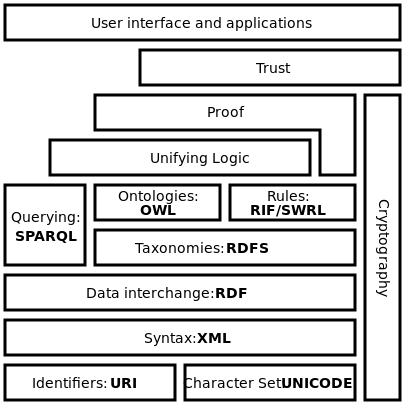
\includegraphics[width=110mm]{Figures/semantic_web_stack.png}
	\caption{The Semantic Web Stack \label{overflow}}
\end{figure}
Hình Semantic Web Stack\cite{semantic3} miêu tả kiến trúc của Semantic Web. Chắc năng mà mối quan hệ giữa các thành phần được tổng hợp lại dưới đây:
\begin{itemize}
\item XML cung cấp một cú pháp cơ bản nhất cho nội dung bên trong tài liệu, và không có liên quan ngữ nghĩa gì đến nội dung ngữ nghĩa mà nội dụng nó chứa. XML không phải là một thành phần cần thiết trong các công nghệ Semantic Web trong hầu hết các trường hợp, tồn tại cú pháp thay thế khác như Turle \textsuperscript{*}. 
\item XML Schema là một ngôn ngữ dùng để cung cấp và hạn chế cấu trúc nội dung của các thành phần nằm trong tài liệu XML, nói cách khác nó giúp chúng ta dạnh nói dung mà tài liệu đó chưa là gì. Ví dụ: OWL/XML vs. RDF/XML
\item RDF \cite{rdf} là một ngôn ngữ đơn giản dùng để diễn tả các mô hình dữ liệu (ở đây muốn chỉ đến các nguồn dữ liệu web) và mối quan hệ của chúng. Một mô hình dự theo RDF có thể được biểu diễn bằng nhiều cú pháp khác nhau, vd: RDF/XML, N3, Turtle và RDFa. Có thể nói RDF chính là thành phần cơ bản và quan trọng nhất của Semantic Web.
\item RDF Schema \cite{rdfs} mở rộng RDF và là từ vựng để đặc tả các thuộc tính và lớp trong các tài nguyên dựa trên RDF, với ngữ nghĩa dựa trên các việc tạo ra nhiều phân cấp lớp và thuộc tính.
\item OWL thêm nhiều từ vựng hơn để diễn các thuộc  tính và lớp, và điểm quan trọng là nó thêm các từ vựng để đặc tả mối quan hệ giữa các lớp với nhau, vd: ranh giới riêng biệt giữa các lớp với nhau (disjointness), các quy định với số lượng (cardinality), cung cấp nhiều loại dữ liệu cho các thuộc tính, và các đặc tính của các thuộc tính (vd: đối xứng/ bất đối xứng, và các lớp liệt kê.
\item SPARQL là một giao thức và ngôn ngữ truy vấn dữ liệu dành cho tài nguyên của semantic web.
\item RIF (W3C Rule Interchange Format) là một ngữ ngữ XML để biểu diễn điều luật web mà máy tính có thể thực thi.
\end{itemize}
{\let\thefootnote\relax\footnotetext{*\textit{
			Turtle: http://en.wikipedia.org/wiki/Turtle\_(syntax)}}
}
\paragraph{Kết luận} Trên đây chúng em chỉ liệt kê những thành phần và tiêu chuẩn cơ bản nhất mà tổ chức W3C đã vạch ra nhằm xây dựng một mô hình Web ngữ nghĩa của tương lai. Nội dung để tài của chúng em chỉ hạn chế trong việc nghiên cứu và khai thác ngôn ngữ ontology web nhằm khai thác tiềm năng về mặc ngữ nghĩa (suy luận ra những thông tin mới dựa trên những suy luận từ ngữ nghĩa của những thông tin được khai báo) nhằm phục vụ cho việc phân loại thông qua các thuộc tính của sản phẩm. Chương kế tiếp sẽ đi qua tìm hiểu về Ontology Web Language(OWL) và Semantic Web Rule Language (SWRL) hai thành phần chính giúp hình thành khả năng phần loại tự động của đề tài này.




